%   Filename    : chapter_4.tex 
\chapter{Preliminary Results/System Prototype}
This chapter presents the results on estimating the depth of potholes using the StereoPi system. It details the prototype construction, calibration of the system, and the application of regression analysis to improve depth estimation. It also contains the measurements taken during the testing phases, comparing the ground truth depths with the value estimated by the camera. Findings are presented systematically, supported by tables showing the collected data, images of the outputs, and discussion on the analysis of results.

\section{System Calibration and Model Refinement}
After the initial testing, the system was calibrated using a controlled setup, where artificial potholes with known depths were created. The stereo camera system captured disparity maps, from which depth was calculated using the standard stereo vision formula:

\[
\text{Depth} = \frac{f \times B}{d}
\]

where:
\begin{itemize}
	\item \( f \) is the focal length in pixels,
	\item \( B \) is the baseline distance between the two cameras,
	\item \( d \) is the disparity.
\end{itemize}


However, preliminary observations revealed that the relationship between measured disparity and true depth was nonlinear, particularly for small disparities corresponding to greater distances. As a result, a direct application of the stereo formula led to systematic errors, especially at the extremes of the depth range.

To address the nonlinear behavior, a curve fitting approach was introduced. Specifically, an inverse model was fitted to the collected data points, relating disparity and ground-truth distance measurements.

An inverse function of the form:

\[
y = a + \frac{b}{x}
\]

where:
\begin{itemize}
	\item \( y \) is the estimated distance (in cm),
	\item \( x \) is the measured disparity,
	\item \( a \) and \( b \) are coefficients obtained through regression analysis.
\end{itemize}

\section{Model Refinement Using Regression}
The regression analysis produced the following model parameters:
\begin{itemize}
	\item a = …
	\item b = ...
\end{itemize}

The model achieved the following performance on the test data:

\begin{table}[H]
	\centering
	\begin{tabular}{|c|c|}
		\hline
		\textbf{Metric} & \textbf{Value} \\ \hline
		Mean Absolute Error (MAE) & X cm \\ \hline
		Root Mean Square Error (RMSE) & X cm \\ \hline
	\end{tabular}
	\caption{Performance Metrics for the Regression Model}
	\label{tab:performance_metrics}
\end{table}

The relatively low MAE and RMSE indicate that the fitted model significantly improved the accuracy of depth estimation compared to the original stereo formula.


\section{Error Analysis}
Despite the improvements, minor estimation errors remained. These errors were primarily attributed to:
\begin{itemize}
	\item Low-light imaging conditions affecting disparity computation,
	\item Shallow potholes with depths less than 3 cm, where disparity resolution becomes a limiting factor,
	\item Perspective distortion when the stereo camera was not parallel to the ground plane.
\end{itemize}


\section{Testing Results}
Following calibration, actual potholes located around the University of the Philippines Visayas (UPV) campus were tested. The ground truth depths of the potholes were measured manually and compared with the depths estimated by the camera. Based on the results, the StereoPi camera was able to estimate the depths fairly close to the ground truth values.The smallest difference was seen in Pothole 5, where the estimated depth was only 0.24 cm away from the ground truth. The largest difference was found in Pothole 1, where the error was 3.45 cm. For the other potholes, the differences were 0.67 cm for Pothole 2, 2.07 cm for Pothole 3, and 2.66 cm for Pothole 4. Most of the time, the camera’s estimated depths were only off by about one to three centimeters. Table \ref{tab:comparison} shows the comparison between the manually measured ground truth depths and the depths estimated by the StereoPi camera for each simulated pothole.

\begin{table}[H]
	\centering
	\hspace{-2cm}
	\small 
	\caption{Ground Truth and StereoPi Depth Measurements}
	\begin{tabular}{|p{1.5cm}|p{1.5cm}|p{1.5cm}|p{1.5cm}|p{1.5cm}|p{1.5cm}|p{1.5cm}|p{1.5cm}|}
		\hline
		\textbf{Pothole} & \textbf{Ground Truth 1 (cm)} & \textbf{Ground Truth 2 (cm)} & \textbf{Ground Truth Avg (cm)} & \textbf{Est Depth 1(cm)} & \textbf{Est Depth 2 (cm)} & \textbf{Est Depth Avg(cm)} & \textbf{Diff(cm)} \\ \hline
		
		1 & 14.6 & 14.4 & 14.5 & 11.16 & 10.94 & 11.05 & 3.45  \\ \hline
		2 & 12.0 & 12.1 & 12.05 & 12.36 & 10.4 & 11.38 & 0.67 \\ \hline
		3 & 6.4 & 6.5 & 6.45 & 4.76 & 4.0 & 4.38 & 2.07 \\ \hline
		4 & 9.8 & 9.3 & 9.55 & 6.16 & 7.62 & 6.89 & 2.66 \\ \hline
		5 & 13.9 & 14.3 & 14.1 & 13.04 & 14.68 & 13.86 & 0.24 \\ \hline
		
	\end{tabular}
	\label{tab:comparison}
	\hspace{-3cm}
\end{table}

\begin{figure}[htbp]
	\centering
	\begin{minipage}{0.32\textwidth}
		\centering
		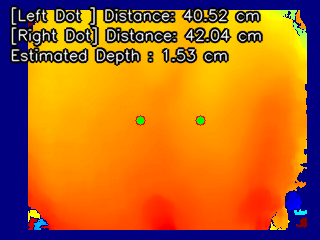
\includegraphics[width=\textwidth]{disparity.png}
		\caption{Disparity Map}
		\label{fig:image1}
	\end{minipage}
	\hfill
	\begin{minipage}{0.32\textwidth}
		\centering
		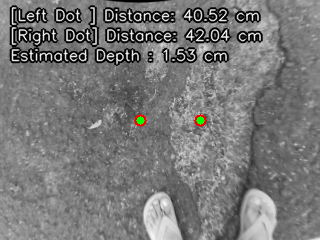
\includegraphics[width=\textwidth]{left.png}
		\caption{Left Stereo Image}
		\label{fig:image2}
	\end{minipage}
	\hfill
	\begin{minipage}{0.32\textwidth}
		\centering
		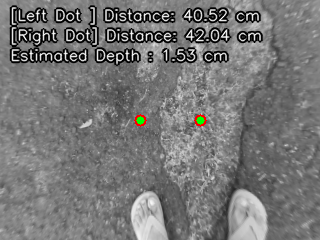
\includegraphics[width=\textwidth]{right.png}
		\caption{Right Stereo Image}
		\label{fig:image3}
	\end{minipage}
\end{figure}



\section{Discussion}

